The experimental setup consisted in an ablation approach to investigate the impact of individual features on the performance of two machine learning algorithms, namely Support Vector Machines (SVM) and XGBoost. To conduct the study, each feature in the feature set (as presented in Table \ref{tab:features}) was removed one at a time, and the models were retrained without the removed feature, as shown in table \ref{tab:ablation}. Subsequently, the performance of the models was evaluated on a validation set, which consisted of 30\% of the training set, with a stratification of the target variable. As the distribution of the target variable was imbalanced, as illustrated in Table \ref{tab:tags}, two sampling techniques were incorporated into the training pipeline. Specifically, the pipeline involved a column preprocessor that implemented standard scaling for numeric features and TF-IDF (term frequency-inverse document frequency) vectorizer, both implementations came from he sklearn library \cite{scikit-learn}. Additionally, two sampling techniques, random oversampling for minority classes and random undersampling for majority classes, were included. The parameters for the grid search consisted of three parameters per algorithm, including "max depth", "col sample by tree", and "learning rate" for XGBoost, and "C", "kernel type", and "$\gamma$" for SVM.

\begin{table}[!ht]
\centering
\caption{\label{tab:ablation} Sets of Features During Ablation}
\begin{tabular}{cl}
\hline
\textbf{Iteration} & \multicolumn{1}{c}{\textbf{Set of Features}} \\
\hline
1 & hasNegAffix, Token, Dependency, Head, NegExpList, $Lemma_{i-1}$, POS, Lemma, RootPath \\
2 & hasNegAffix, Token, Dependency, Head, NegExpList, $Lemma_{i-1}$, Lemma, RootPath \\
3 & hasNegAffix, Dependency, Head, NegExpList, $Lemma_{i-1}$, Lemma, RootPath \\
4 & hasNegAffix, Head, NegExpList, $Lemma_{i-1}$, Lemma, RootPath \\
5 & hasNegAffix, NegExpList, $Lemma_{i-1}$, Lemma, RootPath \\
6 & $Lemma_{i-1}$, Lemma, hasNegAffix, RootPath \\
7 & $Lemma_{i-1}$, hasNegAffix, RootPath \\
8 & $Lemma_{i-1}$, RootPath \\
9 & $Lemma_{i-1}$ \\
\hline
\end{tabular}
\end{table}


\subsection{Support Vector Machine} 
\textbf{SVM} was first introduced by Vapnik and Cortes(1995) \cite{vapnik1995}, and was quickly recognized as one of the most successful classification algorithms. The basic idea behind the model is finding such a hyperplane between the plotted classes in a way, where the margin, i.e. the distance, between the two classes is maximized. SVM algorithms show great robustness against noise and control over-fitting \cite{robust2009}. Moreover, previous work regarding the application of SVM for negation Cue Detection, as described in the Related Work section, suggests the state-of-the-art performance of the algorithm for this task. The specific implementation of SVM used in this paper was  "\textit{thundersvm}", which make use of GPU in its computations. The library was created by Wen Zeyi et al. \cite{thundersvm}


\subsection{XGBoost}
XGBoost is a powerful and complex machine learning algorithm that has shown excellent performance in capturing intricate patterns in data \cite{minasny2009elements}. As a tree-based classifier, it sequentially builds new trees upon the starting predictor tree, with each new tree aiming to predict the margin of error of the decision produced by the ensemble of trees it is built upon \cite{minasny2009elements}.

In the present research, XGBoost's tree-based classifier was implemented with the XGBoost package. The $tree\_method$ parameter was set to $gpu\_hist$ in order to decrease the running time of the algorithm. Specifically, this approach performs sketching only once and makes use of GPU, thereby enhancing computational efficiency.

\FloatBarrier
\subsection{Classification Experiments}

\begin{figure}[!h]
\centering
    \makebox[\textwidth][c]{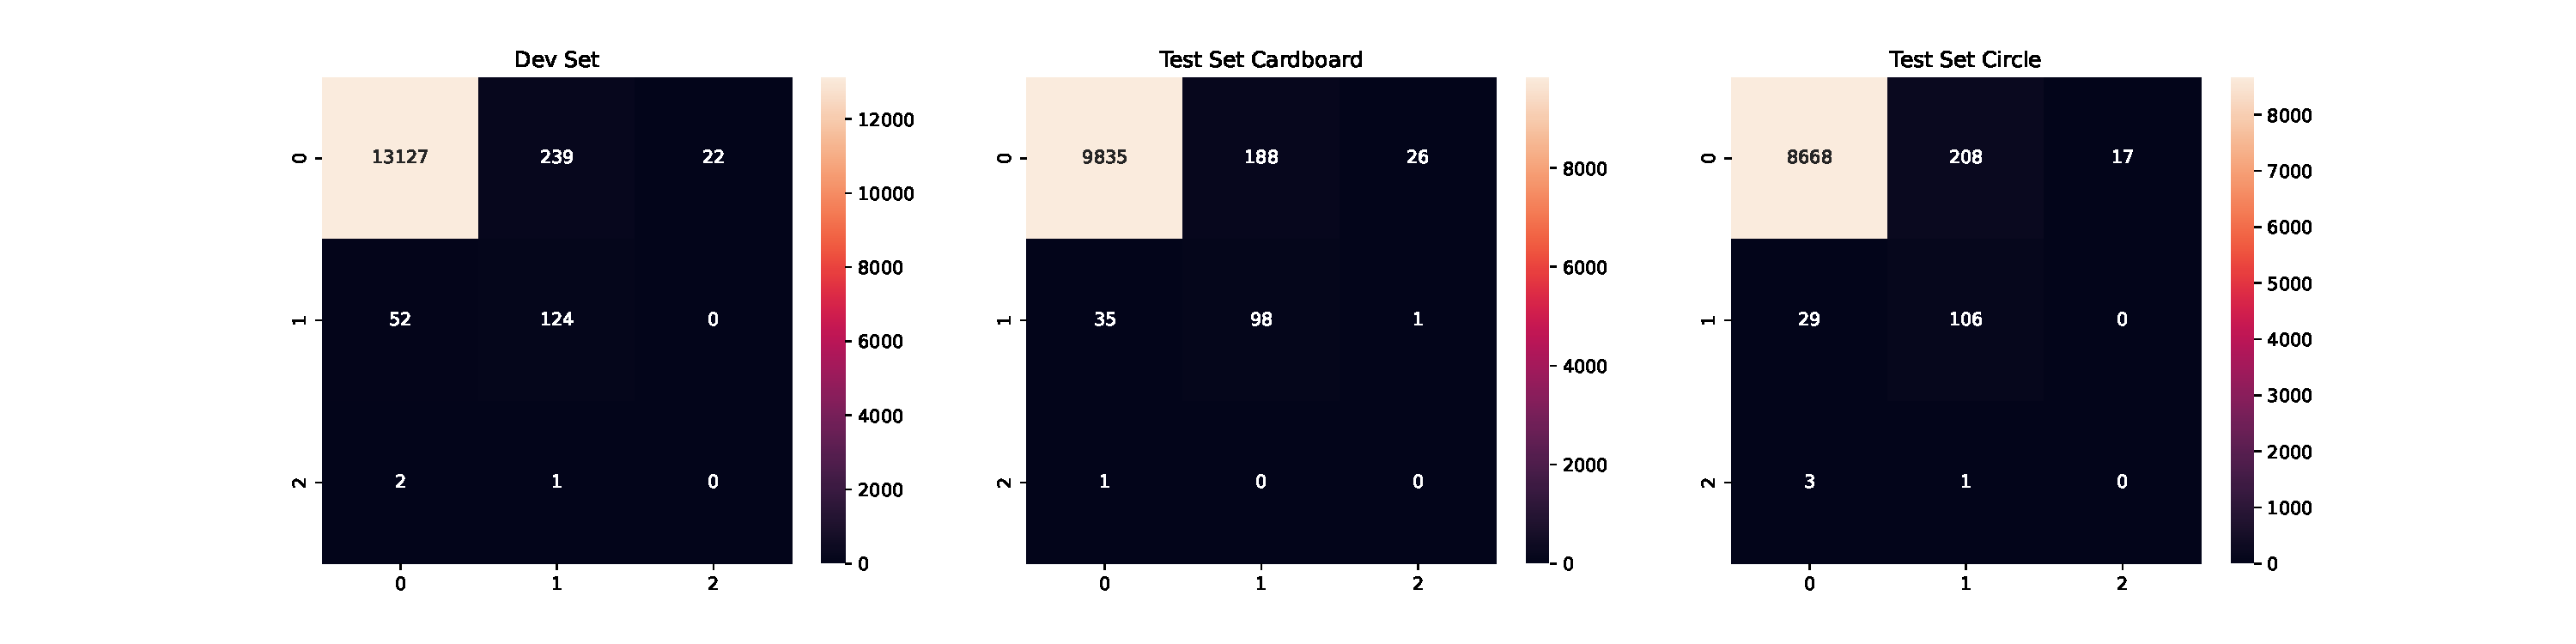
\includegraphics[width=1.3\textwidth]{Plots and results/Confusion_Matrix_svm.pdf}}
  \caption{Confusion Matrices Best Selected SVM}
  \label{fig:base_best_svm}
\end{figure}


\begin{figure}[!ht]
\centering
    \makebox[\textwidth][c]{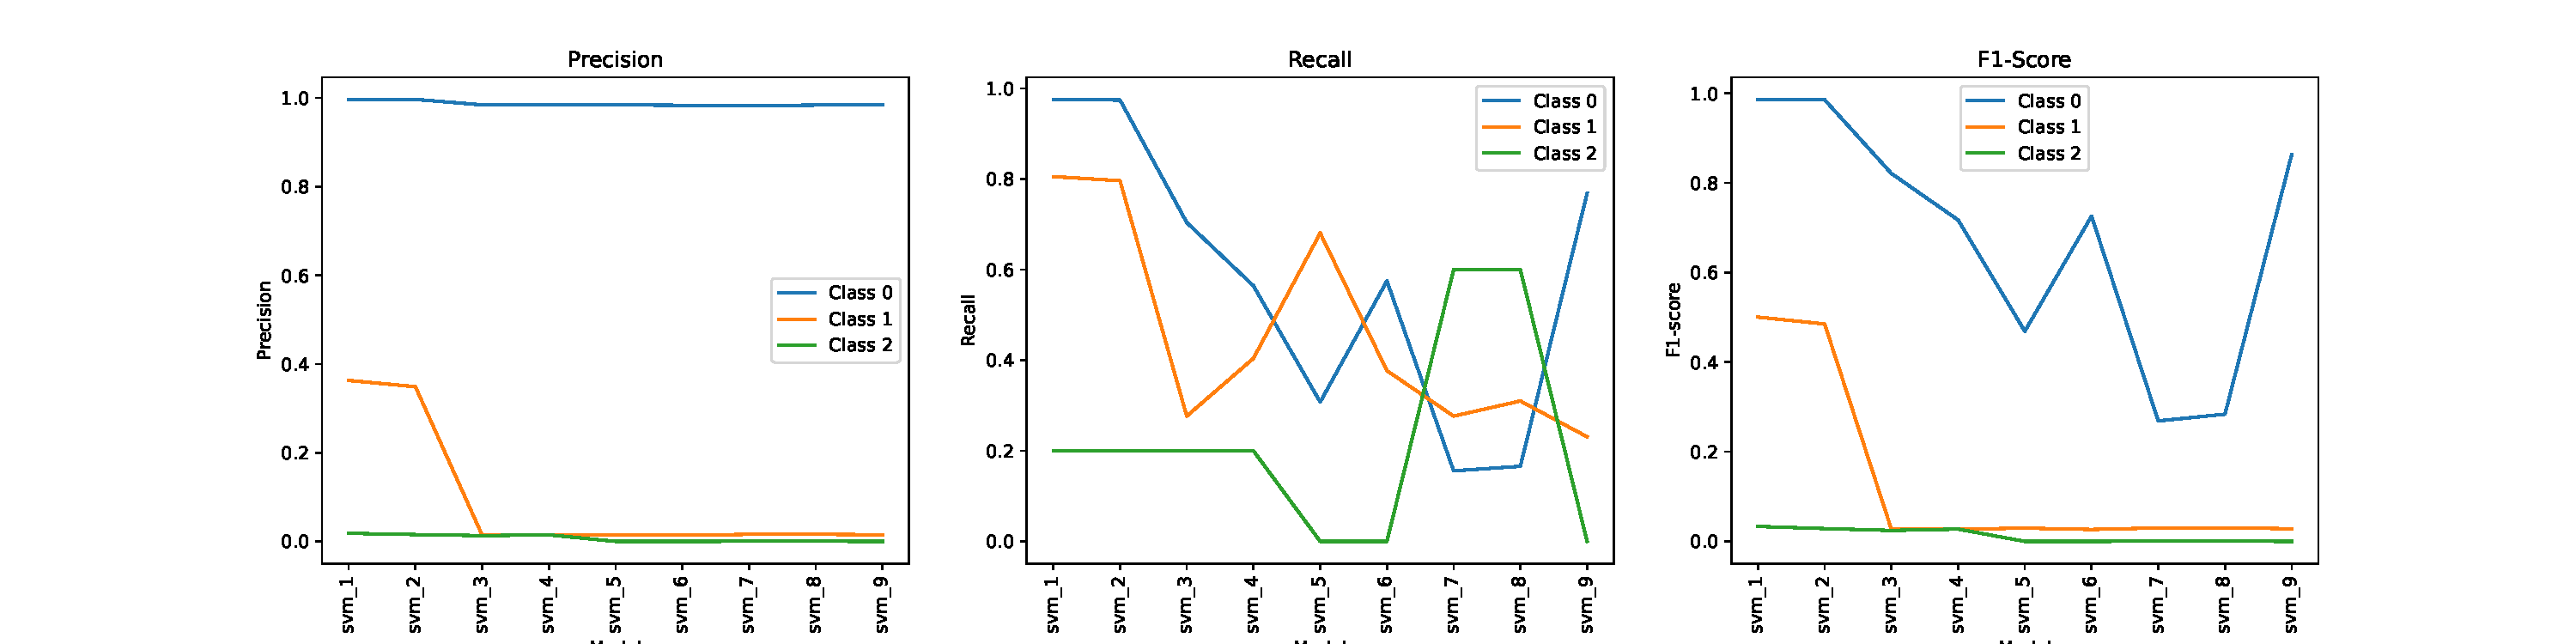
\includegraphics[width=1.3\textwidth]{Plots and results/metrics_svm_training.pdf}}
  \caption{Metrics During Ablation Study SVM}
  \label{fig:metrics_svm_training}
\end{figure}

\begin{table}[!ht]
    \centering
    \caption{Classification Report Best Performing Model}
    \label{tab:results}
\begin{tabular}{lccc|cccr}
\hline
Dataset & \begin{tabular}[c]{@{}l@{}}Precision\\ (SVM)\end{tabular} &    \begin{tabular}[c]{@{}l@{}}Recall\\ (SVM)\end{tabular} &  \begin{tabular}[c]{@{}l@{}}F1-Score\\ (SVM)\end{tabular} & \begin{tabular}[c]{@{}l@{}}Precision\\ (XGBoost)\end{tabular} &    \begin{tabular}[c]{@{}l@{}}Recall\\ (XGBoost)\end{tabular} &  \begin{tabular}[c]{@{}l@{}}F1-Score\\ (XGBoost)\end{tabular} & Support  \\
\hline
\textbf{Cardboard} &        &        &        &       &       &       &    \\
O                  & 0.996  &  0.978 & 0.987  & 0.995 & 0.967 & 0.981 & 10049 \\
B-NEG              &  0.342 &  0.731 &  0.466 & 0.244 & 0.686 & 0.360 & 134 \\
I-NEG              &    0.0 &    0.0 &    0.0 &  0.0  & 0.0   & 0.0   & 1 \\
macro avg          &  0.446 &  0.570 &  0.484 & 0.413 & 0.551 & 0.447 & 10184 \\
weighted avg       &  0.987 &  0.975 &  0.980 & 0.985 & 0.963 & 0.973 & 10184 \\
\hline
\textbf{Circle}    &        &        &        &       &       &       &   \\
O                  &  0.996 &  0.974 &  0.985 & 0.995 & 0.959 & 0.977 & 8893 \\
B-NEG              &  0.336 &  0.785 &  0.471 & 0.220 & 0.718 & 0.337 & 135 \\
I-NEG              &    0.0 &    0.0 &    0.0 &  0.0   & 0.0   &   0.0 & 4 \\
macro avg          &  0.444 &  0.586 &  0.485 & 0.405 & 0.559 & 0.438 & 9032 \\
weighted avg       &  0.986 &  0.971 &  0.9772 & 0.984 & 0.955 & 0.9672 & 9032 \\
\hline
\textbf{Dev set}   &        &        &        &       &       & &   \\
O                  &  0.995 &  0.980 &  0.988 & 0.995 & 0.969 & 0.982 & 13388 \\
B-NEG              &  0.340 &  0.704 &  0.988 & 0.228 & 0.664 & 0.982 & 176 \\
I-NEG              &  0.0   &  0.0   &  0.0   & 0.043 & 0.333 & 0.076 & 3 \\
macro avg          &  0.445 &  0.561 &  0.482 & 0.422 & 0.655 & 0.466 & 13567 \\
weighted avg       &  0.987 &  0.976 &  0.981 & 0.985 & 0.964 & 0.973 & 13567 \\
\hline
\end{tabular}
\end{table}




\begin{figure}[!ht]
\centering
    \makebox[\textwidth][c]{\includegraphics[width=1.3\textwidth]{Plots and results/metrics_xgb_training.pdf}}
  \caption{Metrics During Ablation Study XGBoost}
  \label{fig:metrics_xgb_training}
\end{figure}




\begin{figure}[!h]
\centering
    \makebox[\textwidth][c]{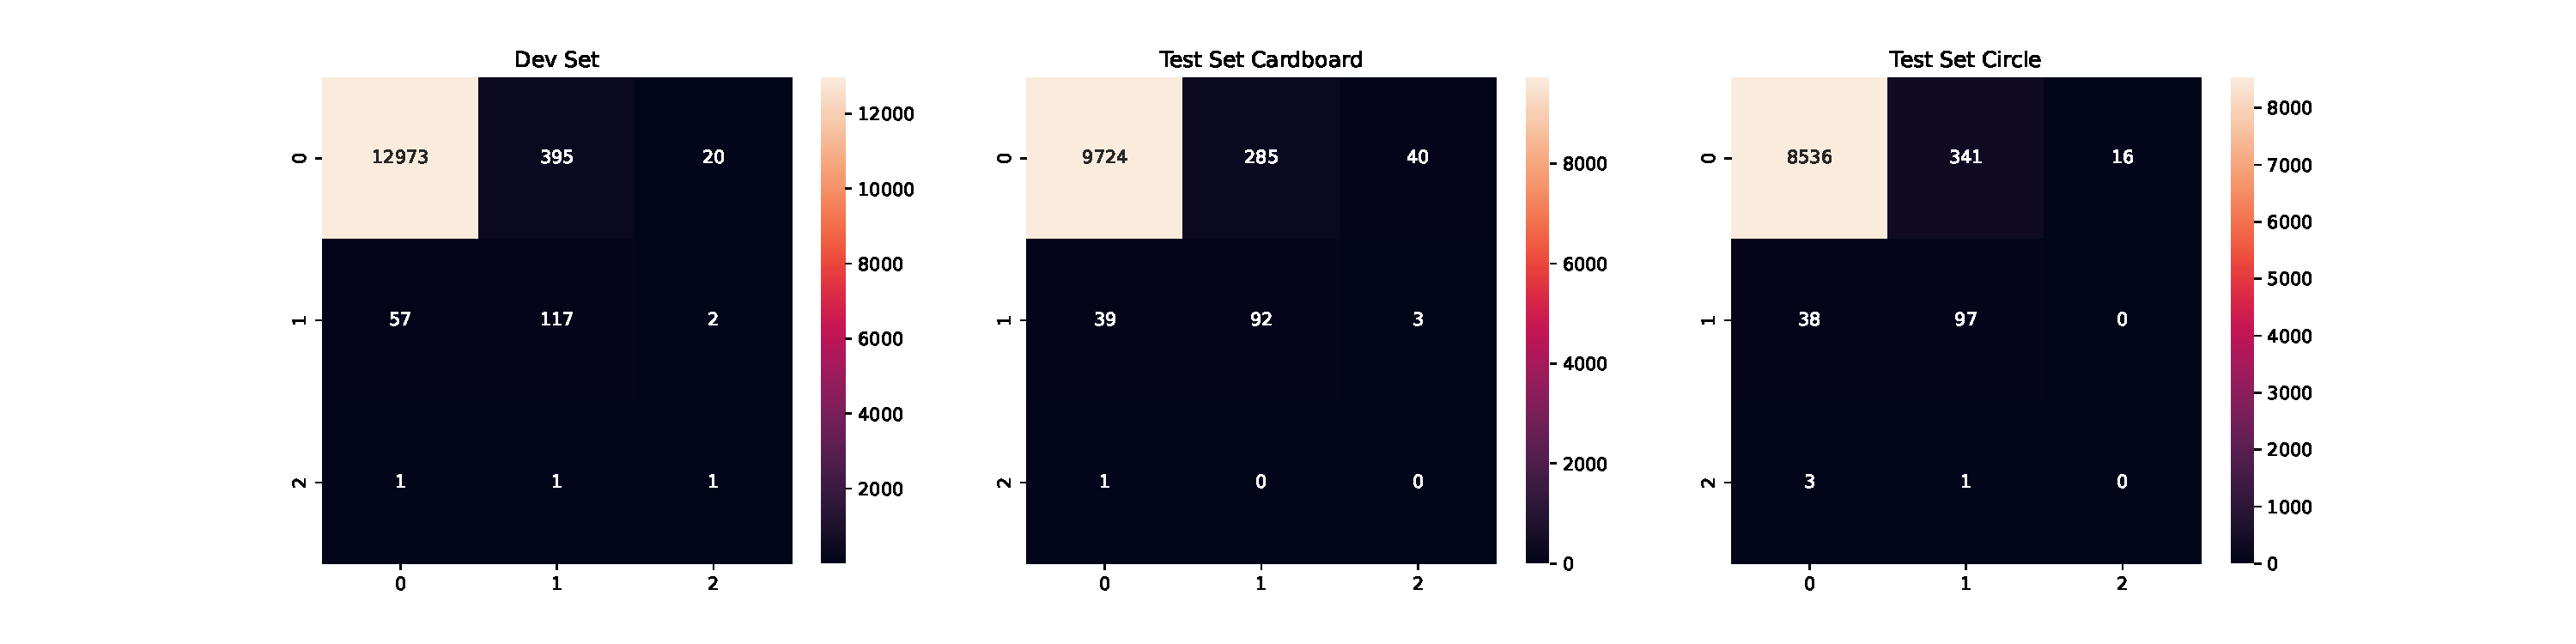
\includegraphics[width=1.3\textwidth]{Plots and results/Confusion_Matrix_xgb.pdf}}
  \caption{Confusion Matrices Best Selected XGBoost}
  \label{fig:base_best_xgb}
\end{figure}












\FloatBarrier
\subsection{Baseline}

\begin{figure}[!ht]
\centering
    \makebox[\textwidth][c]{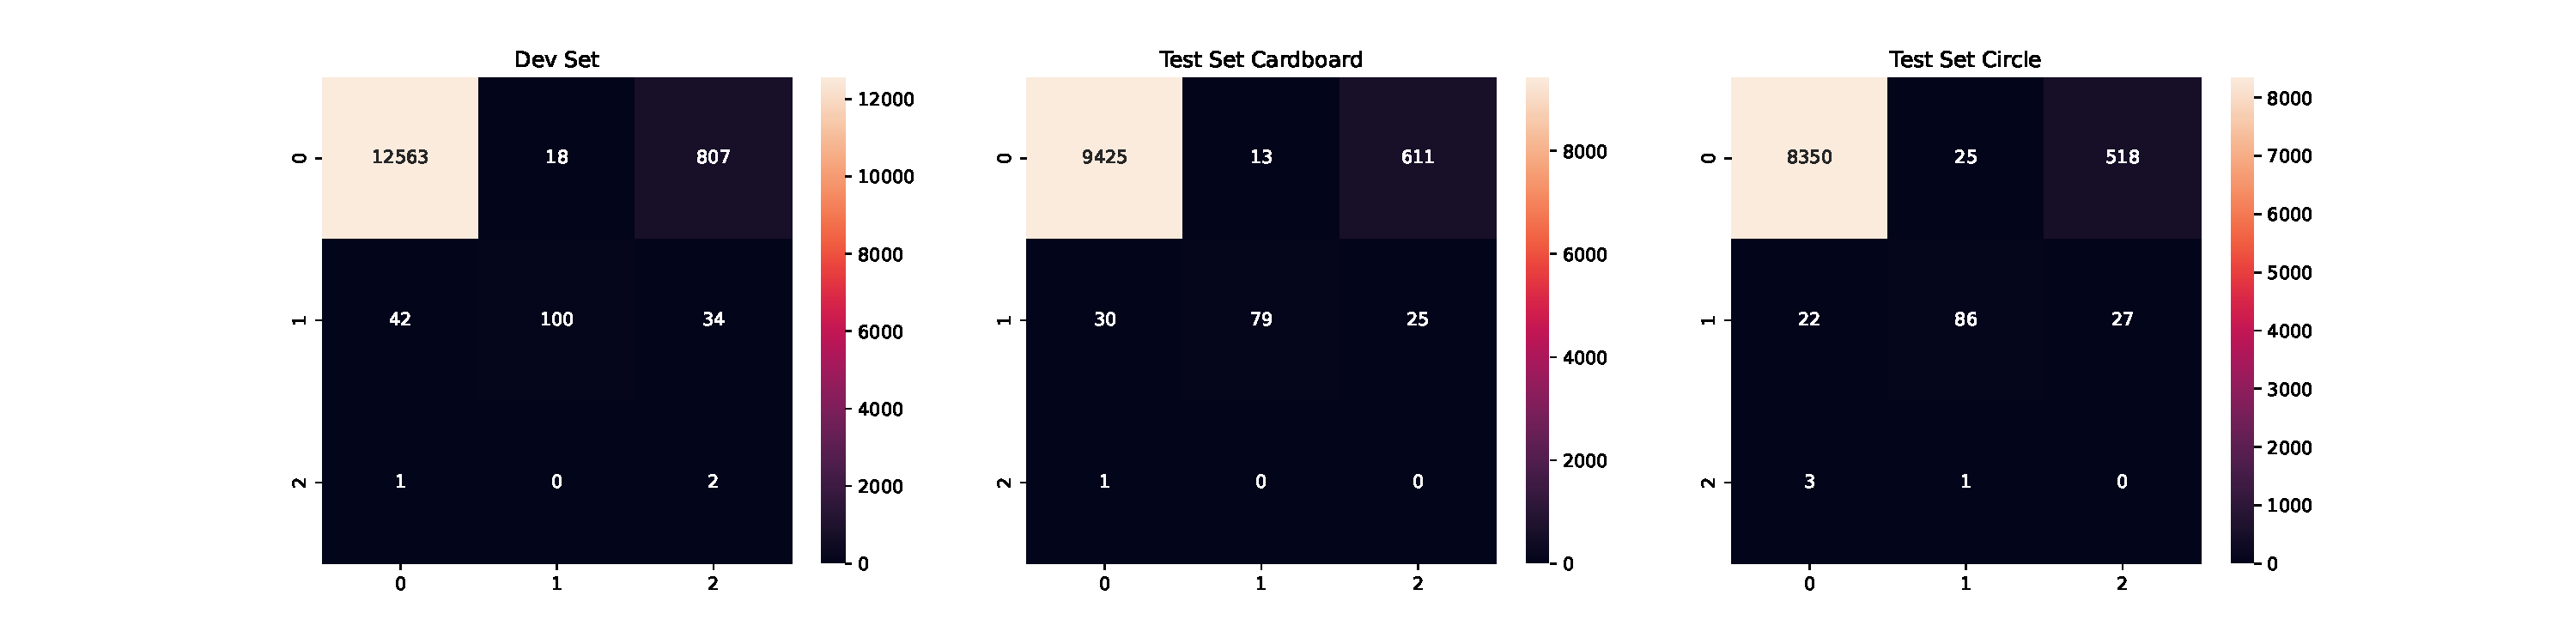
\includegraphics[width=1.3\textwidth]{Plots and results/Confusion_Matrix_base_svm.pdf}}
  \caption{Confusion Matrices Baseline SVM}
  \label{fig:base_line_svm}
\end{figure}


\begin{table}[!ht]
    \centering
    \caption{Classification Report Baseline}
    \label{tab:baselines_results}
\begin{tabular}{lccc|cccr}
\hline
Dataset & \begin{tabular}[c]{@{}l@{}}Precision\\ (SVM)\end{tabular} &    \begin{tabular}[c]{@{}l@{}}Recall\\ (SVM)\end{tabular} &  \begin{tabular}[c]{@{}l@{}}F1-Score\\ (SVM)\end{tabular} & \begin{tabular}[c]{@{}l@{}}Precision\\ (XGBoost)\end{tabular} &    \begin{tabular}[c]{@{}l@{}}Recall\\ (XGBoost)\end{tabular} &  \begin{tabular}[c]{@{}l@{}}F1-Score\\ (XGBoost)\end{tabular} & Support  \\
\hline
\textbf{Cardboard} &        &        &        &       &       &       &    \\
O                  &  0.996 &  0.937 &  0.966 & 0.995 & 0.938 & 0.966 & 10049 \\
B-NEG              &  0.858 &  0.589 &  0.699 & 0.894 & 0.507 & 0.647 & 134 \\
I-NEG              &    0.0 &    0.0 &    0.0 &  0.0  & 0.0   & 0.0   & 1 \\
macro avg          &  0.618 &  0.509 &  0.555 & 0.630 & 0.481 & 0.537 & 10184 \\
weighted avg       &  0.994 &  0.933 &  0.962 & 0.994 & 0.932 & 0.961 & 10184 \\
\hline
\textbf{Circle}    &        &        &        &       &       &       &   \\
O                  &  0.997 &  0.938 &  0.967 & 0.995 & 0.940 & 0.967 & 8893 \\
B-NEG              &  0.767 &  0.637 &  0.696 & 0.850 & 0.548 & 0.667 & 135 \\
I-NEG              &    0.0 &    0.0 &    0.0 &  0.0  & 0.0   &   0.0 & 4 \\
macro avg          &  0.588 &  0.525 &  0.554 & 0.615 & 0.496 & 0.544 & 9032 \\
weighted avg       &  0.993 &  0.934 &  0.962 & 0.992 & 0.934 & 0.962 & 9032 \\
\hline
\textbf{Dev set}   &        &        &        &       &       & &   \\
O                  &  0.996 &  0.938 &  0.966 & 0.995 & 0.939 & 0.966 & 13388 \\
B-NEG              &  0.847 &  0.568 &  0.966 & 0.925 & 0.494 & 0.966 & 176 \\
I-NEG              &  0.002 &  0.667 &  0.004 & 0.002 & 0.667 & 0.004 & 3 \\
macro avg          &  0.615 &  0.724 &  0.550 & 0.641 & 0.700 & 0.538 & 13567 \\
weighted avg       &  0.994 &  0.933 &  0.962 & 0.994 & 0.933 & 0.962 & 13567 \\
\hline
\end{tabular}
\end{table}




\begin{figure}[!h]
\centering
    \makebox[\textwidth][c]{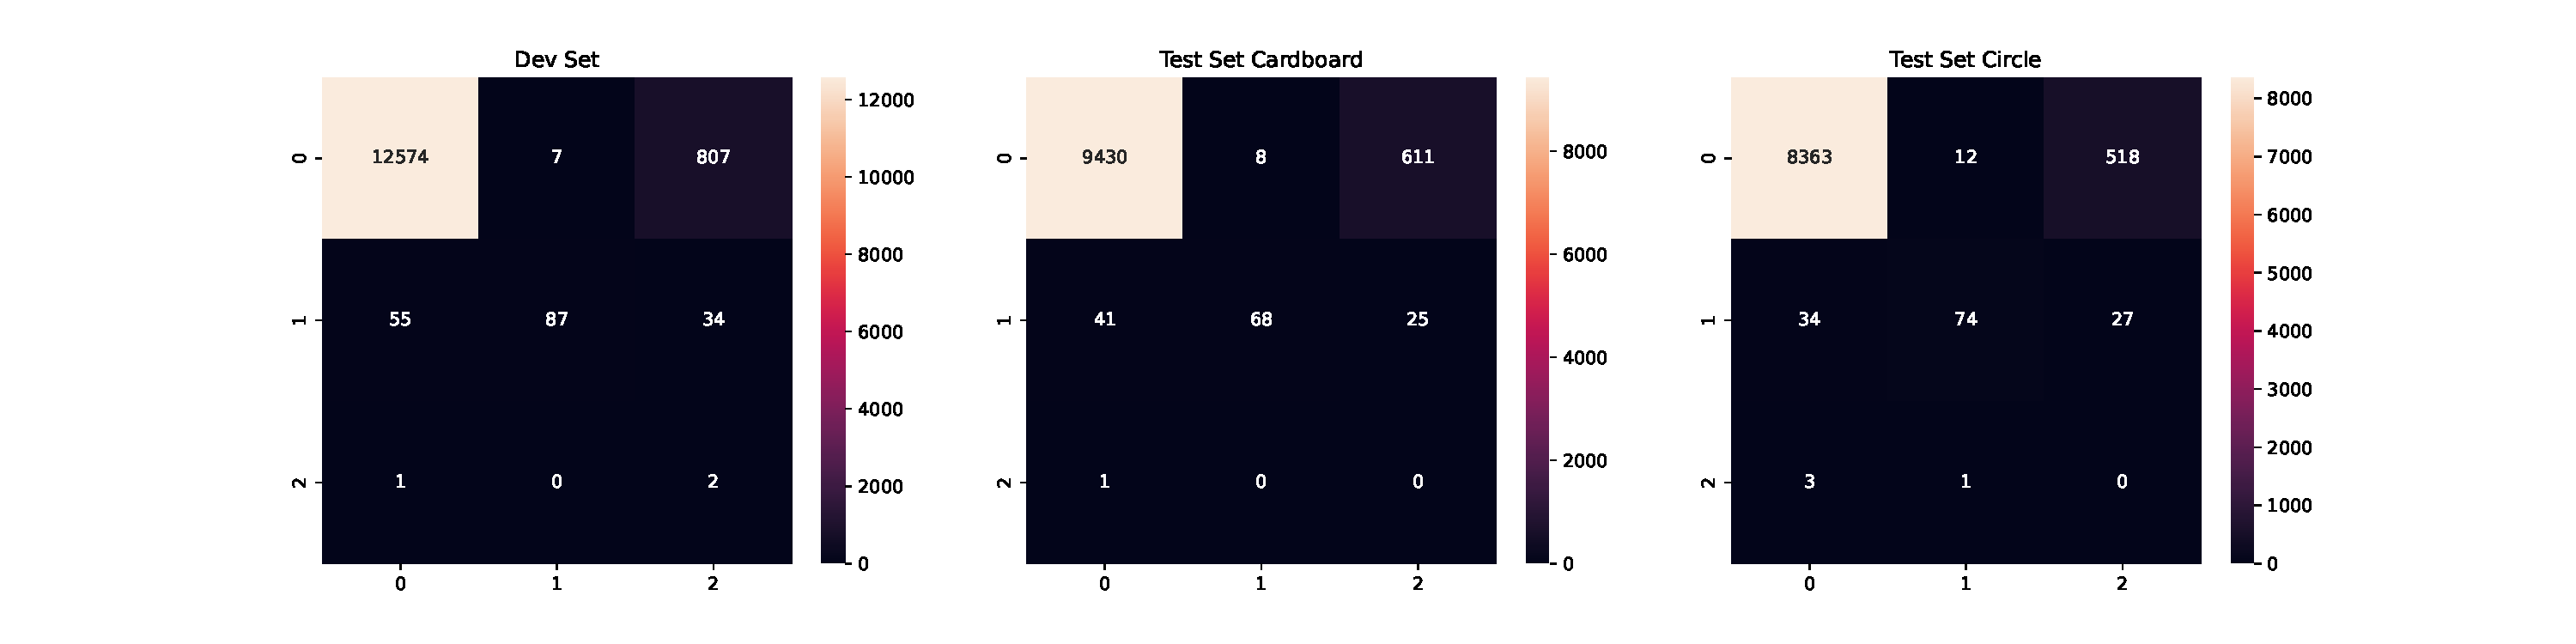
\includegraphics[width=1.3\textwidth]{Plots and results/Confusion_Matrix_base_xgb.pdf}}
  \caption{Confusion Matrices Baseline XGBoost}
  \label{fig:base_line_xgb}
\end{figure}


\FloatBarrier



